\section{Optical pre-processing}\label{sec:optpreproc}

This section presents various pre-processing tasks that are presented in 
a classical order to obtain a calibrated, pan-sharpened image. 

\subsection{Optical radiometric calibration}\label{ssec:optcal}

In remote sensing imagery, pixel values are called DN (for Digital
Numbers) and can not be physically interpreted and compared: they are
influenced by various factors such as the amount of light flowing
trough the sensor, the gain of the detectors and the analogic to
numeric converter.

Depending on the season, the light and atmospheric conditions, the
position of the sun or the sensor internal parameters, these DN can
drastically change for a given pixel (apart from any ground change
effects). Moreover, these effects are not uniform over the spectrum:
for instance aerosol amount and type has usually more impact on the
blue channel.

Therefore, it is necessary to calibrate the pixel values before any
physical interpretation is made out of them. In particular, this
processing is mandatory before any comparison of pixel spectrum
between several images (from the same sensor), and to train a
classifier without dependence to the atmospheric conditions at the
acquisition time.

Calibrated values are called surface reflectivity, which is a ratio
denoting the fraction of light that is reflected by the underlying
surface in the given spectral range. As such, its values lie in the
range $[0,1]$. For convenience, images are often stored in thousandth
of reflectivity, so that they can be encoded with an integer type.
Two levels of calibration are usually distinguished:

\begin{itemize}
\item The first level is called \emph{Top Of Atmosphere (TOA)}
  reflectivity. It takes into account the sensor gain, sensor spectral
  response and the solar illumination.
\item The second level is called \emph{Top Of Canopy (TOC)}
  reflectivity. In addition to sensor gain and solar illumination, it
  takes into account the optical thickness of the atmosphere, the
  atmospheric pressure, the water vapor amount, the ozone amount, as
  well as the composition and amount of aerosol gasses.
\end{itemize}

This transformation can be done either with \app or with
\mont. Sensor-related parameters such as gain, date, spectral
sensitivity and sensor position are seamlessly read from the image
metadata. Atmospheric parameters can be tuned by the user. Supported
sensors are :
\begin{itemize}
\item SPOT5,
\item QuickBird,
\item Ikonos,
\item WorldView1,
\item WorldView2,
\item Formosat.
\end{itemize}

\subsubsection{Optical calibration with \app}

The \application{OpticalCalibration} application
allows to perform optical calibration. The mandatory
parameters are the input and output images. All other parameters are
optional. By default the level of calibration is set to TOA (Top Of 
Atmosphere).  The output images are expressed in thousandth of 
reflectivity using a 16 bits unsigned integer type.

A basic TOA calibration task can be performed with the following command :

\begin{verbatim}
otbcli_OpticalCalibration -in  input_image -out output_image
\end{verbatim}

A basic TOC calibration task can be performed with the following command :

\begin{verbatim}
otbcli_OpticalCalibration -in  input_image -out output_image -level toc
\end{verbatim}

\subsubsection{Optical calibration with \mont}

These transformations can also be done in \mont.

The 6S model needs atmospheric parameters to be able to compute
radiative terms to estimate the atmospheric contributions on the input
signal. Default parameters are available in the module.  For
atmospheric parameters, it is possible to indicate AERONET file. The
AERONET (AErosol RObotic NETwork) program is a federation of
ground-based remote sensing aerosol networks established by NASA and
PHOTONS (Univ. of Lille 1, CNES, and CNRS-INSU) and is greatly
expanded by collaborators from national agencies, institutes,
universities, individual scientists, and partners. The program
provides accessible public domain database of aerosol optical,
mircrophysical and radiative properties.

The module produces four outputs:

\begin{itemize}
\item Luminance image.
\item TOA reflectance image.
\item TOC reflectance image.
\item Difference TOA-TOC image, which allows to get the estimation of atmospheric contribution.
\end{itemize}

\begin{figure}
  \center
  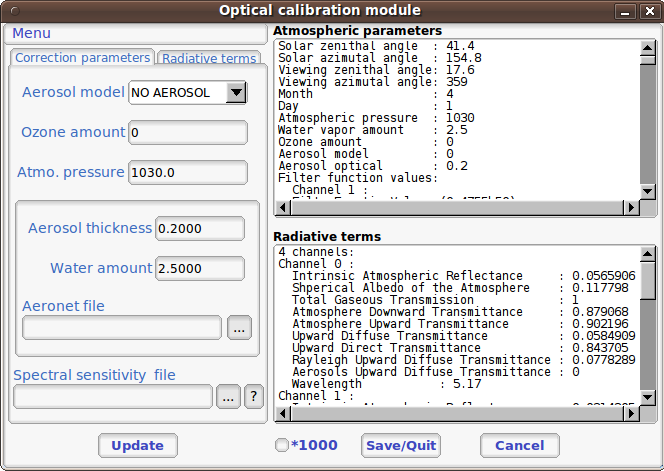
\includegraphics[width=0.6\textwidth]{../Art/MonteverdiImages/monteverdi_optical_calibration.png}
  \itkcaption[GUI of the optical calibration module based on the 6S model]{Optical calibration module.}
  \label{fig:opticalcalibration}
\end{figure}


\begin{figure}
  \center
  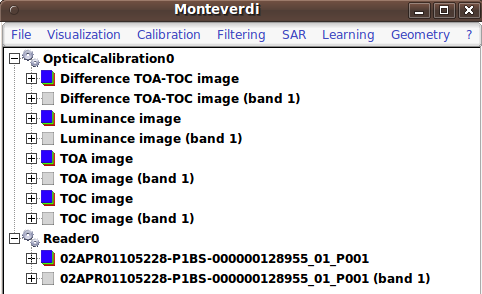
\includegraphics[width=0.6\textwidth]{../Art/MonteverdiImages/monteverdi_optical_calibration_outputs.png}
  \itkcaption[Output of the optical calibration module]{Optical calibration module's outputs.}
  \label{fig:opticalcalibrationoutput}
\end{figure}

\subsection{Pan-sharpening}\label{ssec:pxs}

Because of physical constrains on the sensor design, it is difficult
to achieve high spatial and spectral resolution at the same time : a
better spatial resolution means a smaller detector, which in turns
means lesser optical flow on the detector surface. On the contrary,
spectral bands are obtained through filters applied on the detector
surface, that lowers the optical flow, so that it is necessary to
increase the detector size to achieve an acceptable signal to noise
ratio.

For these reasons, many high resolution satellite payload are composed
of two sets of detectors, which in turns delivers two different kind
of images :

\begin{itemize}
\item The multi-spectral (XS) image, composed of 3 to 8 spectral bands
  containing usually blue, green, red and near infra-red bands at a
  given resolution (usually from 2.8 meters to 2 meters).
\item The panchromatic (PAN) image, which is a grayscale image acquired by a
  detector covering a wider part of the light spectrum, which allows
  to increase the optical flow and thus to reduce pixel
  size. Therefore, resolution of the panchromatic image is usually
  around 4 times lower than the resolution of the multi-spectral image
  (from 46 centimeters to 70 centimeters).
\end{itemize}

It is very frequent that those two images are delivered side by side
by data providers. Such a dataset is called a bundle. A very common
remote sensing processing is to fuse the panchromatic image with the
multi-spectral one so as to get an image combining the spatial
resolution of the panchromatic image with the spectral richness of the
multi-spectral image. This operation is called pan-sharpening.

This fusion operation requires two different steps :
\begin{enumerate}
\item The multi-spectral (XS) image is zoomed and registered to the
  panchromatic image,
\item A pixel-by-pixel fusion operator is applied to the co-registered
  pixels of the multi-spectral and panchromatic image to obtain the
  fused pixels.
\end{enumerate}

Using either \app or modules from \mont, it is
possible to perform both steps in a row, or step-by-step fusion, as
described in the above sections.

\subsubsection{Pan-sharpening with \app}

The \application{BundleToPerfectSensor} application allows to
perform both steps in a row. Seamless sensor modelling is used to
perform zooming and registration of the multi-spectral image on the
panchromatic image. Then, a simple pan-sharpening is applied,
according to the following formula:

\begin{equation}
PXS(i,j) = \frac{PAN(i,j)}{PAN_{smooth}(i,j)} \cdot XS(i,j)
\end{equation}

Where $i$ and $j$ are pixels indices, $PAN$ is the panchromatic image,
$XS$ is the multi-spectral image and $PAN_{smooth}$ is the
panchromatic image smoothed with a kernel to fit the multi-spectral
image scale.

Here is a simple example of how to use the
\application{BundleToPerfectSensor} application:

\begin{verbatim}
otbcli_BundleToPerfectSensor -inp pan_image -inxs xs_image -out output_image
\end{verbatim}

There are two more optional parameters that can be useful for this
tool:
\begin{itemize}
\item The \verb?-elev? option allows to specify the elevation, either with
  a DEM formatted for OTB (\verb?-elev.dem.path? option, see 
  section~\ref{ssec:dem}) or with an average elevation (\verb?-elev.average.value? 
  option). Since registration
  and zooming of the multi-spectral image is performed using
  sensor-models, it may happen that the registration is not perfect in
  case of landscape with high elevation variation. Using a DEM in this
  case allows to get better registration (see \ref{ssec:registration}
  to learn about how to lower registration error).
\item The \verb?-lmSpacing? option allows to specify the step of the
  registration grid between the multi-spectral image and panchromatic
  image. This is expressed in amount of panchromatic pixels. A lower
  value gives a more precise registration but implies more computation
  with the sensor models, and thus increase the computation
  time. Default value is 10 pixels, which gives sufficient precision
  in most of the cases.
\end{itemize}

Pan-sharpening is a quite heavy processing requiring a lot of system
resource. The \verb?-ram? option allows you to limit the amount of memory
available for the computation, and to avoid overloading your
computer. Increasing the available amount of RAM may also result in
better computation time, seems it optimises the use of the system
resources. Default value is 256 Mb.


\subsubsection{Pan-sharpening with \mont}

\mont allows to perform step-by-step fusion. The followings screenshots highlight operations needed to perform Pan-Sharpening.

\begin{itemize}
\item Open panchromatic and multispectral images in monteverdi using the \mmod{Open Dataset} module or using the  \verb?-il? option of the \mont executable.

\item The \mmod{Superimpose} module is used to zoomed and registered
  the multispectral on the panchromatic image. As a result, we get a
  multispectral dataset with the same geographic extension and the
  same resolution as the panchromatic image, cf ~\ref{fig:qbmulsuper}.

\begin{figure}
  \center
  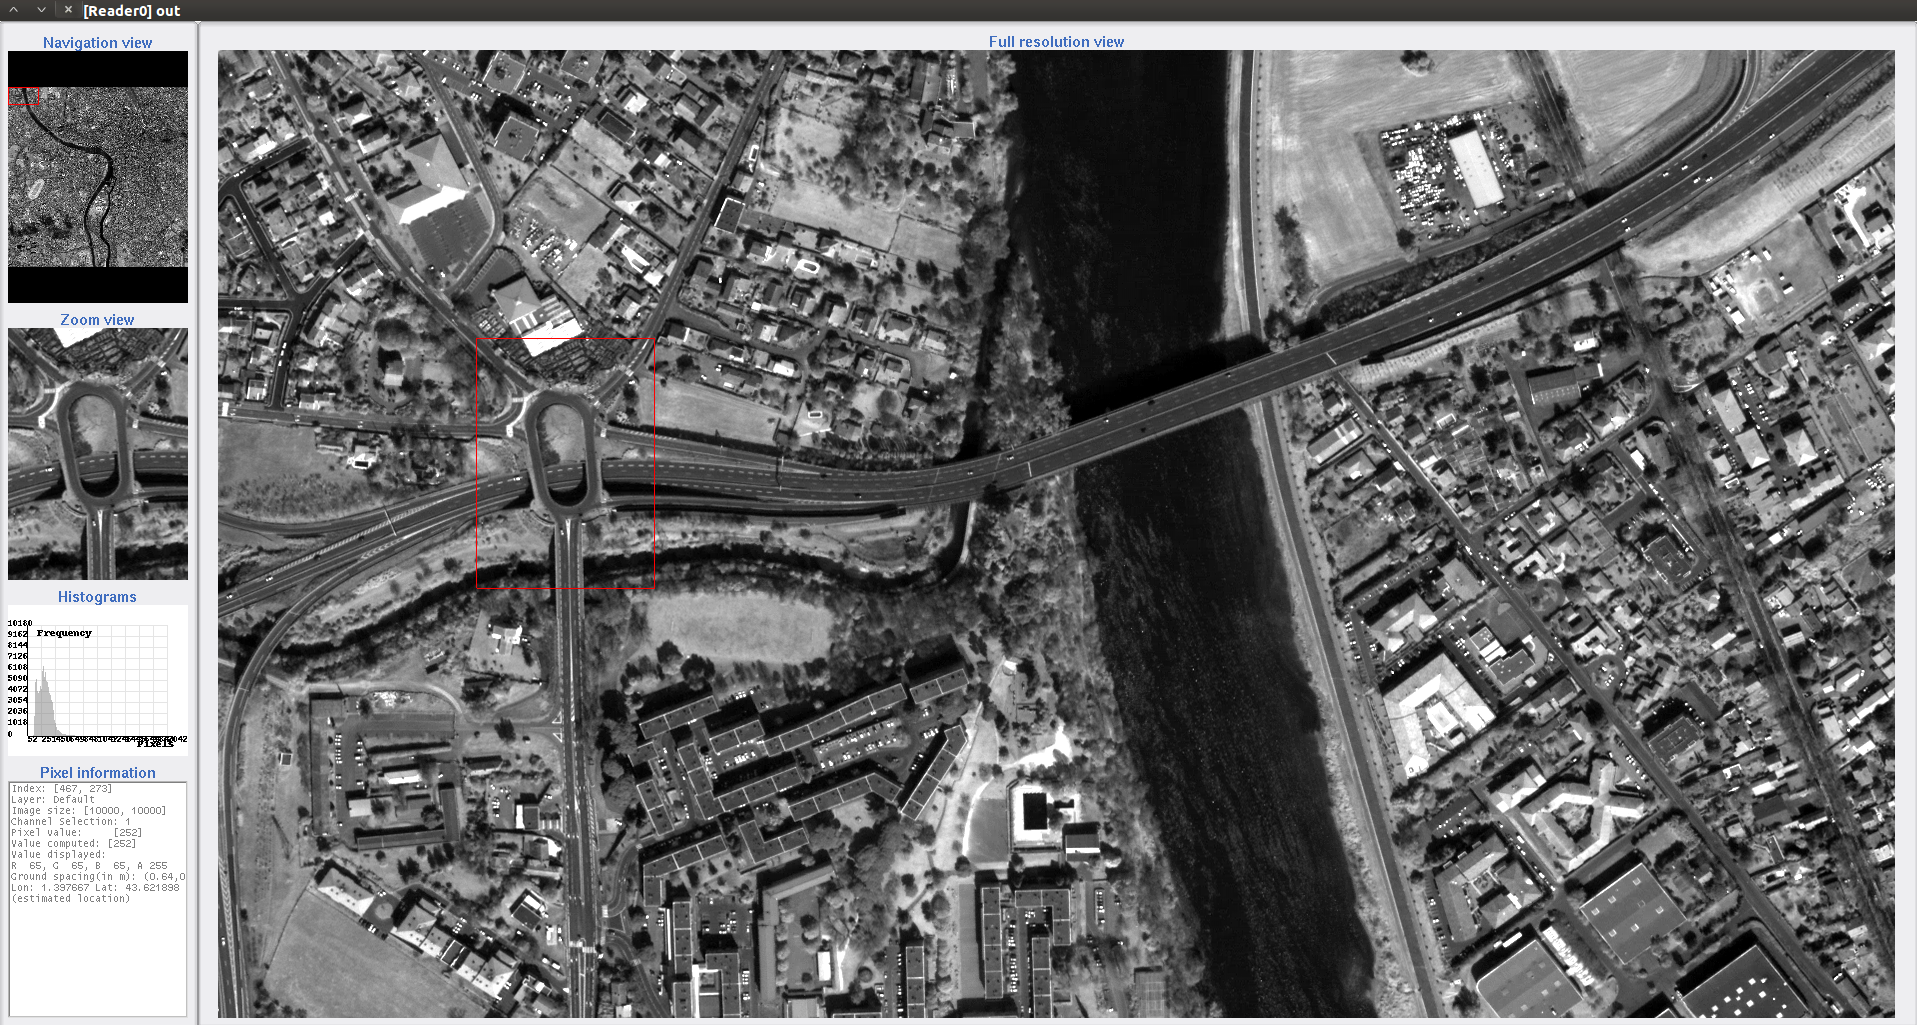
\includegraphics[width=0.45\textwidth]{../Art/MonteverdiImages/monteverdi_QB_PAN_ROI.png}
  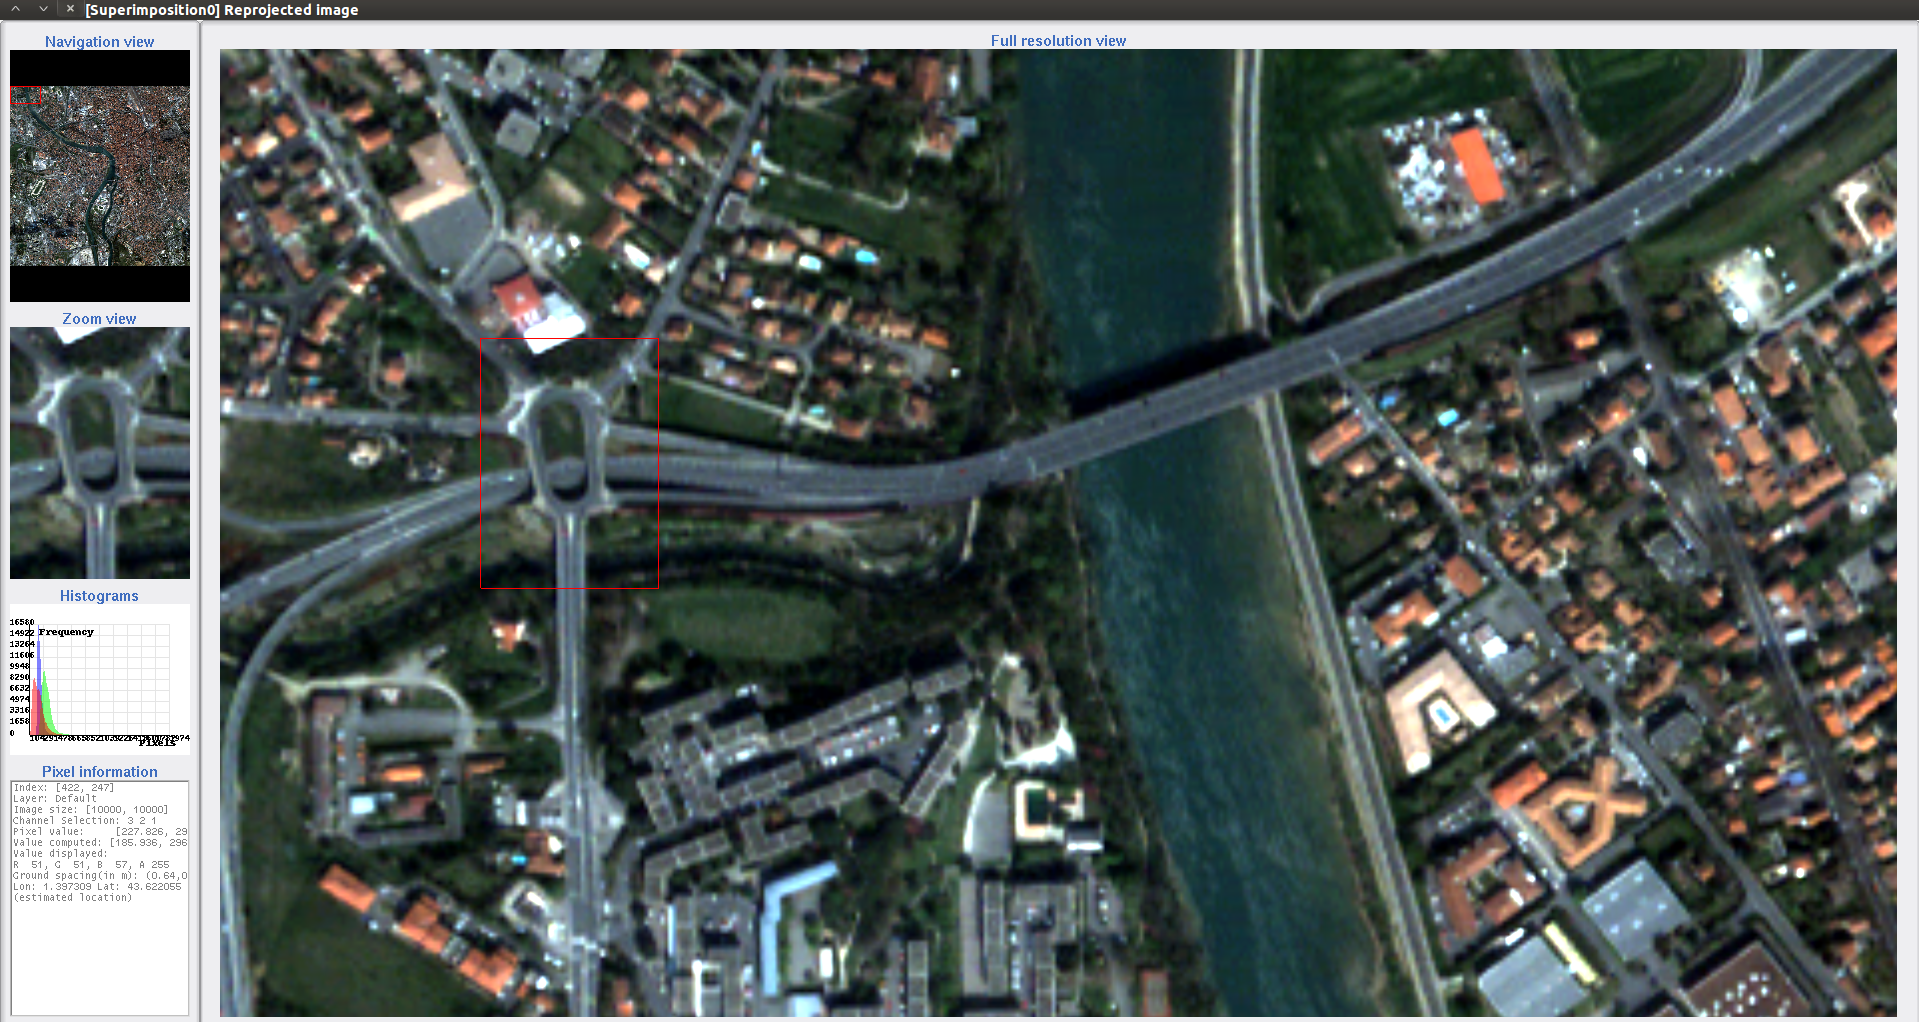
\includegraphics[width=0.45\textwidth]{../Art/MonteverdiImages/monteverdi_QB_MUL_Superimpose.png}
  \itkcaption[Input panchromatic and zoomed and registered multispectral image over it]{Panchromatic, Zoomed, and registered multispectral image.}
  \label{fig:qbmulsuper}
\end{figure}

\item Now the \mmod{Simple RCS pan-sharpening} module can be used using the panchromatic and the multispectral images as inputs. It produces a multispectral image with the same resolution and geographic extension (cf ~\ref{fig:pansharpen}).

\begin{figure}
  \center
  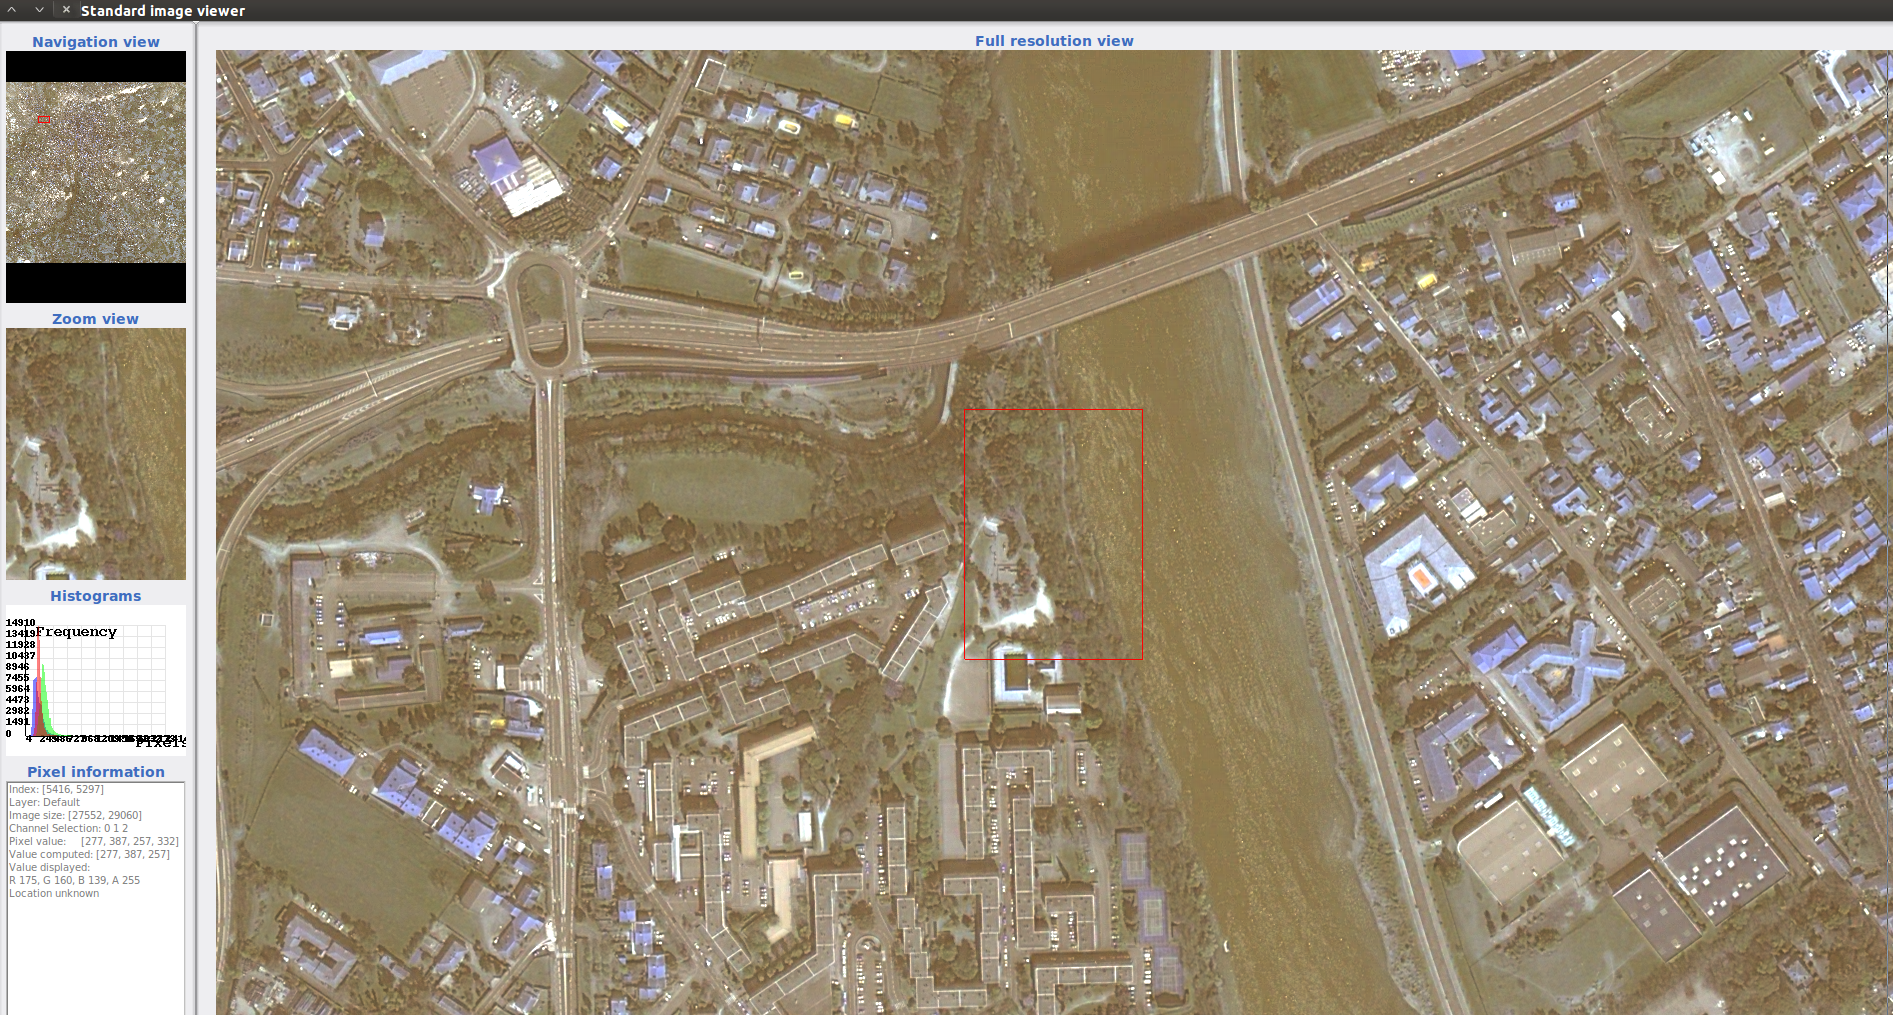
\includegraphics[width=0.6\textwidth]{../Art/MonteverdiImages/monteverdi_QB_XS_pan-sharpened.png}
  \itkcaption[Pan-sharpened image]{Pan-sharpened image using the simple RCS module.}
  \label{fig:pansharpen}
\end{figure}

\end{itemize}


Please also note that since registration and zooming of the
multi-spectral image with the panchromatic image relies on sensor
modelling, this tool will work only for images whose sensor models is
available in \otb (see section~\ref{ssec:ortho} for a detailed
list). It will also work with ortho-ready products in cartographic
projection.

\subsection{Digital Elevation Model management}\label{ssec:dem}

A Digital Elevation Model (DEM) is an georeferenced image (collection
of images) of the elevation. DEM are useful for tasks involving sensor
to ground and ground to sensor coordinate transforms like
ortho-rectification (see section~\ref{ssec:ortho}). In facts, these
transforms need to find the intersection between the line of sight of
the sensor and the earth geoid. If a simple spheroid is used as the
earth model, potentially high localisation errors can be made in areas
where elevation is high or perturbed. Of course, DEM accuracy and
resolution have a great impact on the precision of these transforms.

There exists two main available DEM free of charges with worldwide
cover, which are both delivered as 1-by-1 tiles:
\begin{itemize}
\item \href{http://www2.jpl.nasa.gov/srtm/}{The Shuttle Radar
  topographic Mission (SRTM)} is a 90 meters resolution DEM, obtained
  by radar interferometry during a campaign of the Endeavour space
  shuttle from NASA in 2000.
\item The \href{http://www.ersdac.or.jp/GDEM/E/2.html}{Advanced
  Spaceborne Thermal Emission and Reflection Radiometer (ASTER)} is a
  30 meters resolution DEM obtained by stereoscopic processing of the
  archive of the ASTER instrument.
\end{itemize}

The \otb suite relies on \ossim capabilities for sensor modelling and
DEM handling. Tiles of a given DEM are supposed to be located within a
single directory. Whenever some applications or modules from
\mont require a DEM, there is an option or a field to set the DEM
directory.

%
%\subsubsection{Making DEM files usable in \otb suite using \application{DEMConvert}}
%
%Georeferenced files containing elevation data (including file from
%SRTM and ASTER) need to be converted to a specific file format before
%being compatible with \ossim and \otb. The
%\application{DEMConvert} application allows to perform this
%conversion with the following command:
%
%\begin{verbatim}
%otbcli_DEMConvert -in input_image -out output_prefix
%\end{verbatim}
%
%The output files can then be placed in the directory containing DEM
%files.
%

%\subsubsection{Extract the DEM image corresponding to your image using
%  \mont}


\subsection{Ortho-rectification and map projections}\label{ssec:ortho}

There are several level of products available on the remote sensing
imagery market. The most basic level often provide the geometry of
acquisition (sometimes called the raw geometry). In this case, pixel
coordinates can not be directly used as geographical positions. For
most sensors (but not for all), the different lines corresponds to
different acquisition times and thus different sensor positions, and
different rows correspond to different cells of the detector.

The mapping of a raw image so as to be registered to a cartographic
grid is called ortho-rectification, and consist in inverting the
following effects (at least):
\begin{itemize}
\item In most cases, lines are orthogonal to the sensor trajectory,
 which is not exactly (and in some case not at all) following a
 north-south axis,
\item Depending on the sensor, the line of sight may be different from
  a Nadir (ground position of the sensor), and thus a projective
  warping may appear,
\item The variation of height in the landscape may result in severe
  warping of the image.
\end{itemize}

Moreover, depending on the area of the world the image has been
acquired on, different map projections should be used.

The ortho-rectification process is as follows: once an appropriate map
projection has been defined, a localisation grid is computed to map
pixels from the raw image to the ortho-rectified one. Pixels from the
raw image are then interpolated according to this grid in order to
fill the ortho-rectified pixels.

Ortho-rectification can be performed either with \app or \mont. Sensor
parameters and image meta-data are seamlessly read from the image
files without needing any user interaction, provided that all
auxiliary files are available. The sensor for which \otb
supports ortho-rectification of raw products are the following:
\begin{itemize}
\item SPOT5,
\item Ikonos,
\item Quickbird,
\item GeoEye,
\item WorldView.
\end{itemize}

In addition, GeoTiff and other file format with geographical
information are seamlessly read by \otb, and the ortho-rectification
tools can be used to re-sample these images in another map projection.

\subsubsection{Ortho-rectification with \app}

The \application{OrthoRectification} application allows to
perform ortho-rectification and map re-projection. The simplest way to
use it is the following command:
\begin{verbatim}
otbcli_OrthoRectification -io.in input_image -io.out output_image
\end{verbatim}

In this case, the tool will automatically estimates all the necessary
parameters:
\begin{itemize}
\item The map projection is set to UTM (a worldwide map projection)
  and the UTM zone is automatically estimated,
\item The ground sampling distance of the output image is computed to
  fit the image resolution,
\item The region of interest (upper-left corner and size of the image)
  is estimated so as to contain the whole input image extent.
\end{itemize}

In order to use a Digital Elevation Model (see section~\ref{ssec:dem})
for better localisation performances, one can pass the directory
containing the DEM tiles to the application:

\begin{verbatim}
otbcli_OrthoRectification -io.in input_image 
                          -io.out output_image 
                          -elev dem
                          -elev.dem.path dem_dir
\end{verbatim}

If one wants to use a different map projection, the \emph{-map}
option may be used (example with \emph{lambert93} map projection):

\begin{verbatim}

otbcli_OrthoRectification -io.in input_image 
                          -io.out output_image 
                          -elev dem
                          -elev.dem.path dem_dir 
                          -map lambert93

\end{verbatim}

Map projections handled by the application are the following
(please note that the ellipsoid is always WGS84):
\begin{itemize}
\item UTM : \verb?-map utm? \\
The UTM zone and hemisphere can be set by the options \verb?-map.utm.zone? and \verb?-map.utm.northhem?.
\item Lambert 2 etendu: \verb?-map lambert2?
\item Lambert 93: \verb?-map lambert93?
\item TransMercator: \verb?-map transmercator? \\
The related parameters (false easting, false northing and scale factor) can be set by the 
options \verb?-map.transmercator.falseeasting?, \verb?-map.transmercator.falsenorthing? and 
\verb?-map.transmercator.scale?
\item WGS : \verb?-map wgs?
\item Any map projection system with an EPSG code : \verb?-map epsg? \\
The EPSG code is set with the option \verb?-map.epsg.code?
\end{itemize}

The group \verb?outputs? contains parameters to set the origin, size and spacing of the output image.
For instance, the ground spacing can be specified as follows:

\begin{verbatim}

otbcli_OrthoRectification -io.in input_image 
                          -io.out output_image 
                          -elev dem
                          -elev.dem.path dem_dir 
                          -map lambert93 
                          -outputs.spacingx spx 
                          -outputs.spacingy spy

\end{verbatim}

Please note that since the y axis of the image is bottom oriented, the
y spacing should be negative to avoid switching north and south direction.

A user-defined region of interest to ortho-rectify can be specified as
follows:

\begin{verbatim}

otbcli_OrthoRectification -io.in input_image 
                          -io.out output_image 
                          -elev dem 
                          -elev.dem.path dem_dir 
                          -map lambert93 
                          -outputs.spacingx spx 
                          -outputs.spacingy spy 
                          -outputs.ulx ul_x_coord 
                          -outputs.uly ul_y_coord 
                          -outputs.sizex x_size 
                          -outputs.sizey y_size

\end{verbatim}

Where the \verb?-outputs.ulx? and \verb?-outputs.uly? options allow to 
specify the coordinates of the upper-left corner of the output image.
The \verb?-outputs.sizex? and \verb?-outputs.sizey? options allow to 
specify the size of the output image.

A few more interesting options are available:
\begin{itemize}
\item The \verb?-opt.rpc? option allows to use an estimated RPC model
  instead of the rigorous SPOT5 model, which speeds-up the processing,
\item The \verb?-opt.gridspacing? option allows to define the spacing of the
  localisation grid used for ortho-rectification. A coarser grid
  results in speeding-up the processing, but with potential loss of
  accuracy. A standard value would be 10 times the ground spacing of 
  the output image.
\item The \verb?-interpolator? option allows to change the interpolation
  algorithm between nearest neighbor, linear and bicubic. Default is nearest 
  neighbor interpolation, but bicubic should be fine in most cases.
\item The \verb?-opt.ram? option allows to specify the amount of memory
  available for the processing (in Mb). Default is 256 Mb. Increasing
  this value to fit the available memory on your computer might
  speed-up the processing.
\end{itemize}

%\subsubsection{Ortho-rectification with \mont}
%todo

%\subsection{Residual registration}\label{ssec:registration}
%todo.
